\documentclass[10pt,a4paper]{report}
\usepackage{norme}

% Dossier des images : \includegraphics{mecanique/gabarit.pdf}
\graphicspath{{images/}}

% --- Informations du document -----------------------------------
\NormeTitre{Normes techniques}
\NormeSousTitre{Construction de modules HOm}
\NormeAuteur{Damien De Pascale}
\NormeVersion{0.1}
% La date du jour est utilisée par défaut. Pour la fixer :
% \NormeDate{19.07.2026}

% Pour ne compiler que certains chapitres pendant la rédaction :
% \includeonly{chapitres/01-dessins-schemas}

\begin{document}

\NormePageTitre
\tableofcontents
% \listoffigures   % liste des figures (optionnelle)

% Un fichier par chapitre ; chaque fichier commence par \Chapitre{...}
\Chapitre{Introduction}

\section{But}

Ce document regroupe les normes et les recommandations concernant la fabrication de modules de maquette ferroviaire à l’échelle HOm utilisée par Frédéric et Damien.

\section{Nomenclature}

% TODO changer ce système de numérotation par des symboles ou des couleurs 

Les normes sont repérées par le chiffre 1. 
Elles doivent être respectées pour que les installations soient compatibles.

Les recommandations techniques sont repérées par le chiffre 2. 
Elles servent à simplifier la construction, le montage et l'utilisation des installations.

Les recommandations de réalisme sont repérées par le chiffre 3.
\Chapitre{Structure}

\section{Dimensions}

Les modules doivent s'inscrire dans un volume de base 1200x600 ou 1200x400.

\section{Pieds}

\subsection{Position}

Les modules doivent posséder au minimum 4 fixation pour pied.

Les fixations sont généralement positionnées aux coins du module.
Il faut veiller à ce que les fixations et leurs pied correspondant n'interfèrent pas avec l'interface standard. 
Il faut également veiller à ce que la place suffise pour visser et dévisser les pieds aisément.

Les fixations sont fabriquées selon le dessin correspondant.

\subsection{Fabrication}

Les pieds sont fabriqués selon le dessin correspondant.

Matière première, Tubes de 16x10 en aluminium pressé ou filée selon prix et disponibilité.

Typiquement article 114550 chez Metallica

Bouchon en plastique typiquement BN1099.1409131 de Bossard


\Chapitre{Raccordement}

\section{Principe}

Les réseaux sont constituer de groupe de modules. 
Aux extrémités de ces groupe, se trouve une interface de raccordement standard. 
De cette manière les groupe sont interchangeable. 
Mais les modules à l'intérieur de ces groupes ne le sont pas forcément. 

Les interfaces à l'interne des groupes de modules correspondent aux interfaces standard sauf pour l’emplacement de la voie et le décors.

\section{Interface standard}

Les interfaces standard correspondent au dessin suivant.

Sur les modules de plus de 400mm de large, l'axe de la voie est pris comme référence.
L'axe de la voie doit être au minimum à 200mm du bord du module.

Les interfaces standard sont à des hauteurs définies.
% TODO préciser les hauteurs exactes des interfaces standard

\subsection{Protection voie}

Si des protections pour la voie sont prévues, elles doivent suivre le dessin correspondant.
% TODO faire le dessin

\section{Raccordement électrique}

Les modules de pleine voie sont équipés de 2 bus d'alimentation : l'alimentation traction pour la voie et une alimentation pour les accessoires.

Sur le module vue de face,

Les fils doivent être suffisamment long pour se connecter à une prise sur le module voisin à 200mm du bord avec un rebord de 100mm.

Si le rebord du module est plus haut que 100mm un trou doit être fait pour passer les fils.

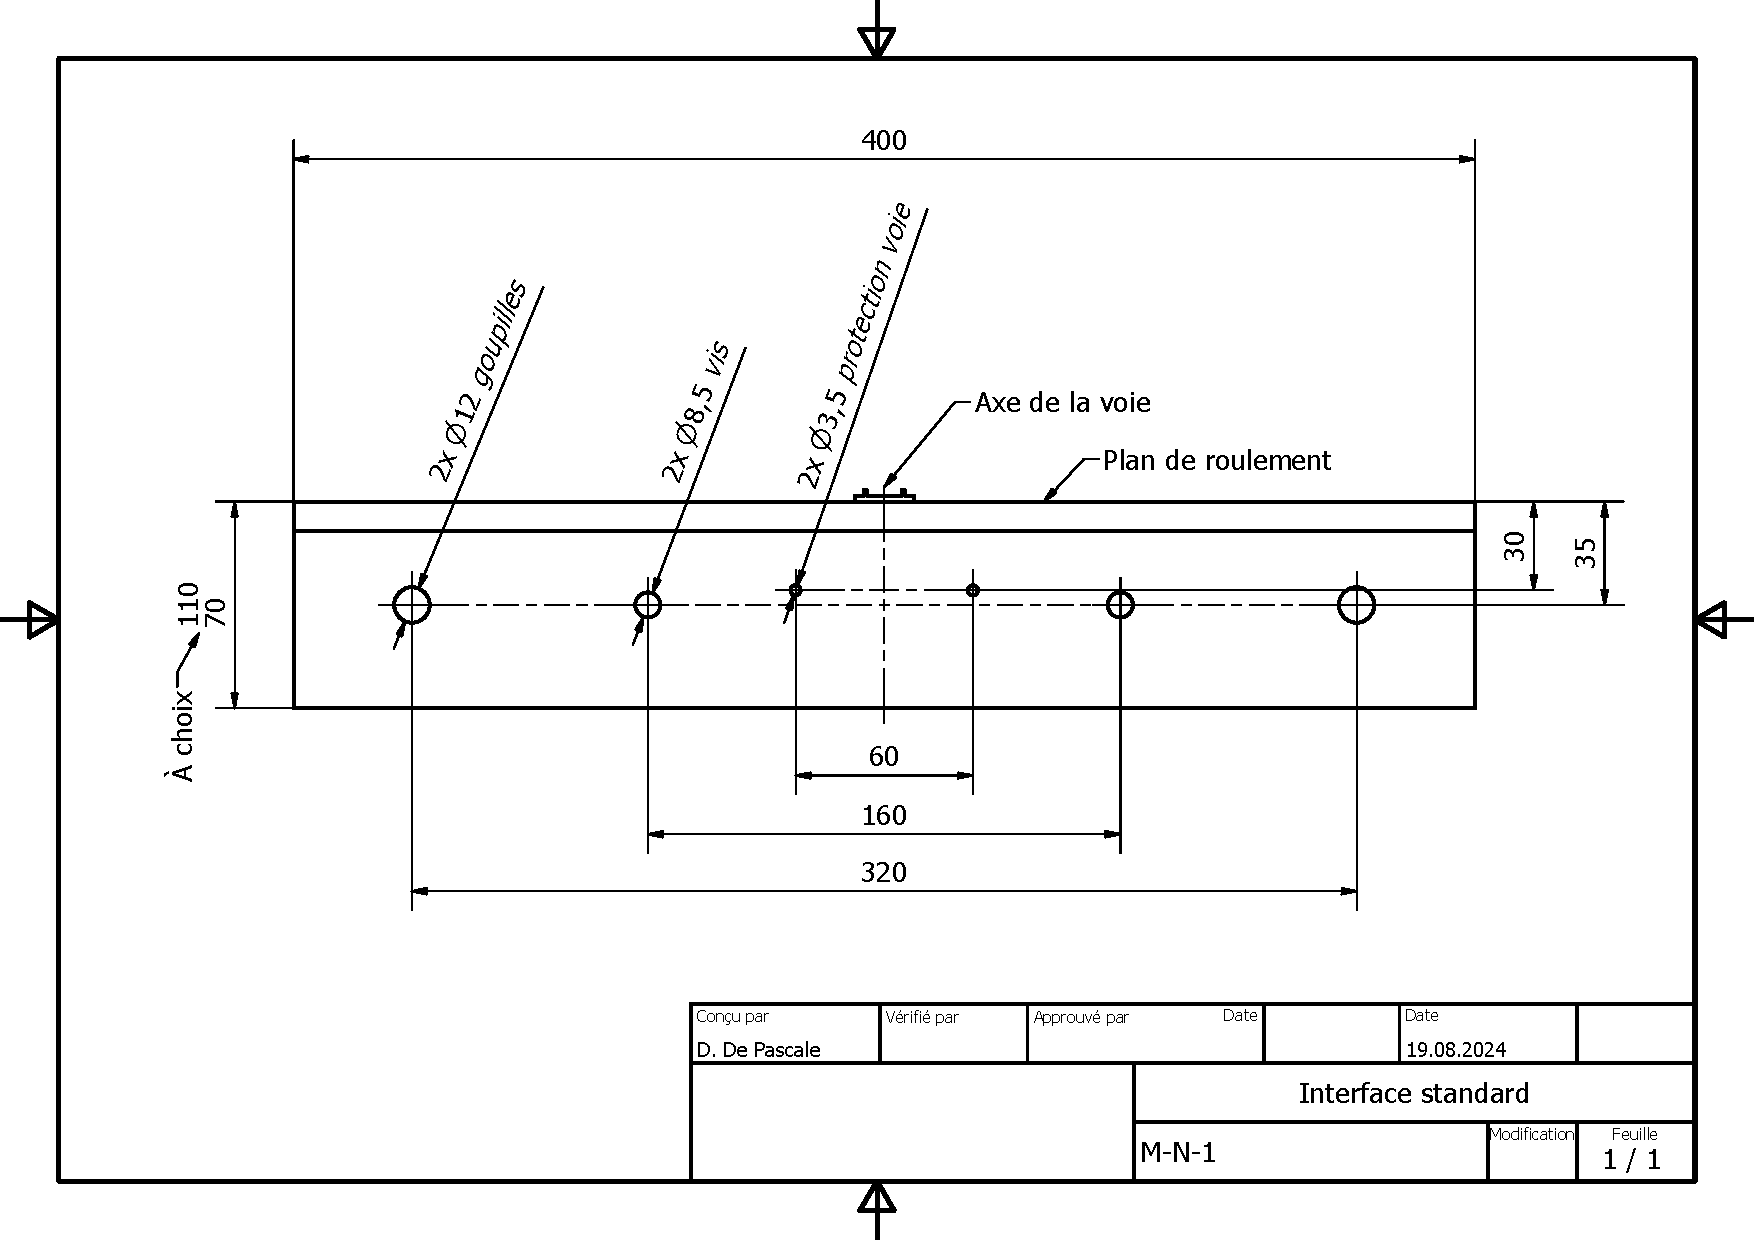
\includepdf[pages=-, fitpaper=true]{images/mecanique/M-N-I40.pdf}
% TODO remplacer "plan de roulement" par le bon nom.
\Chapitre{Câblage}

\section{Couleurs}


\Chapitre{Voies}

\section{Matériel}

La voie peco HOm est utilisée.

Les éclisses isolantes de peco sont utilisées.

Les éclisses conductrices N de minitrix sont utilisées.



\Chapitre{Traction}

\section{Généralités}

La traction est analogique.

\section{Zone d'arrêt signal d'entrée}

Les entrées des gares doivent posséder une zone d'arrêt du signal d'entrée. 
Cette zone d'arrêt doit faire au moins 600mm de long. 
Elle doit commencer au moins 200mm en amont du signal et finir au droit du signal ou plus loin. 
Si la zone d'arrêt se termine en aval du signal, la limite entre la zone d'arrêt est la traction de la gare doit-être repérable par le chef-circulation. 

La zone d'arrêt doit être active (hors tension) au moins dans le sens de l'entrée et être alimenté par le potentiel de la pleine voie. 
Le rail de droite dans le sens d'entrée doit être hors tension.

Entre la zone d'arrêt et la traction de la gare les 2 rails doivent être isolé galvaniquement.

\section{Voie de gare}

Le retour traction est toujours fait par le rail du même côté.

Le retour traction est du côté du pupitre.

\section{Pleine voie}

La pleine voie est décrite dans les normes du block.

% TODO Déplacer dans normes du block
Les pupitres des gares doivent posséder un potentiomètre pour la gestion de la vitesse de chaque pleine voie. 
[voir pour mettre dans les normes du block]
\Chapitre{Décors}


\Chapitre{Étiquetage}

\section{Modules}

Sur les modules, les inscriptions sont faites sur chacune des faces de raccord

Les inscriptions contiennent :

\begin{itemize}
    \item le propriétaire
    \item le n° du module
    \item le n° de sa caisse de rangement
    \item son emplacement de rangement dans la caisse, généralement l'étage
\end{itemize}

% TODO prévoir des couleurs pour chaque indications

\section{Caisses de modules}

Sur les caisses de module, les inscriptions sont faites au minimum sur une des faces et sur le couvercle.

Les inscriptions contiennent :

\begin{itemize}
    \item le propriétaire
    \item le n° de la caisse
    \item la liste des modules disposé de manière similaire à l'emplacement des modules dans la caisse
    \item le poids de la caisse pleine en kg
    \item la hauteur de la caisse
\end{itemize}

Les inscriptions peuvent également contenir :

\begin{itemize}
    \item le nom de la gare ou du groupe de module pour lequel la caisse est nécessaire
    \item la liste des caisses qui sont nécessaire de prendre avec
    \item le lieu de stockage de la caisse
    \item les information de contact du propriétaire
\end{itemize}

\section{caisse de matériel}

Sur les caisses de matériel empilables, les inscriptions sont faites au minimum sur le devant et sur un des côté.

Les inscriptions contiennent :

\begin{itemize}
  \item le propriétaire
  \item le n° de la caisse
  \item la liste ou la désignation générale du contenu
  \item le poids de la caisse pleine en kg
\end{itemize}

Les inscriptions peuvent également contenir :

\begin{itemize}
  \item le nom de la gare ou du groupe de module pour lequel la caisse est nécessaire
  \item la liste des caisses qui sont nécessaire de prendre avec
  \item le lieu de stockage de la caisse
  \item les information de contact du propriétaire
\end{itemize}


\end{document}
